\documentclass[11pt,letterpaper]{article}

\usepackage{fontspec}
\setmainfont{FreeSerif}

\usepackage{fullpage}
\usepackage{graphicx}
\usepackage{amsfonts,eucal,amsbsy,amsopn,amsmath}
\usepackage{url}
\usepackage[sort&compress]{natbib}
\usepackage{natbibspacing}
\usepackage{latexsym}
\usepackage{wasysym} 
\usepackage{rotating}
\usepackage{fancyhdr}
\DeclareMathOperator*{\argmax}{argmax}
\DeclareMathOperator*{\argmin}{argmin}
\usepackage{sectsty}
\usepackage[dvipsnames,usenames]{color}
\usepackage{multicol}
\definecolor{orange}{rgb}{1,0.5,0}
\usepackage{multirow}
\usepackage{sidecap}
\usepackage{caption}
\renewcommand{\captionfont}{\small}
\setlength{\oddsidemargin}{-0.04cm}
\setlength{\textwidth}{16.59cm}
\setlength{\topmargin}{-0.04cm}
\setlength{\headheight}{0in}
\setlength{\headsep}{0in}
\setlength{\textheight}{22.94cm}
\allsectionsfont{\normalsize}
\newcommand{\ignore}[1]{}
\newenvironment{enumeratesquish}{\begin{list}{\addtocounter{enumi}{1}\arabic{enumi}.}{\setlength{\itemsep}{-0.25em}\setlength{\leftmargin}{1em}\addtolength{\leftmargin}{\labelsep}}}{\end{list}}
\newenvironment{itemizesquish}{\begin{list}{\setcounter{enumi}{0}\labelitemi}{\setlength{\itemsep}{-0.25em}\setlength{\labelwidth}{0.5em}\setlength{\leftmargin}{\labelwidth}\addtolength{\leftmargin}{\labelsep}}}{\end{list}}

\bibpunct{(}{)}{;}{a}{,}{,}
\newcommand{\nascomment}[1]{\textcolor{blue}{\textbf{[#1 --NAS]}}}


\pagestyle{fancy}
\lhead{}
\chead{}
\rhead{}
\lfoot{}
\cfoot{\thepage~of \pageref{lastpage}}
\rfoot{}
\renewcommand{\headrulewidth}{0pt}
\renewcommand{\footrulewidth}{0pt}


\title{11-712:  NLP Lab Report}
\author{Jonathan Barker}
\date{April 26, 2013}

\begin{document}
\maketitle
\begin{abstract}
This a report on the development of HindiMorph, an open source morphological analyzer for Hindi. Hindi is a morphologically rich language for which I have created an analyzer. I present a brief background on the language and the phenomena I hope to analyze. Existing work on and tools for Hindi morphology are then reviewed. After that I explain the system design and document my progress, results and ideas for future work. 
\end{abstract}

HindiMorph is an open source morphological analyzer for the Hindi language. Being a morphologically rich language, Hindi may be easier to work with when it's morphemes are tagged instead of just using the surface forms found in text. This report provides a brief introduction to the Hindi language and covers the morphological phenomina that HindiMorph hopes to analyze, in addition to summarizing previous work and other existing tools. It also documents the design of the system as well as it's development and performance.

\section{Basic Information about Hindi}
According to \cite{ethnologue}, Hindi (also Khadi Boli or Khari Boli) is an Indo-European language from India that is spoken by 181,676,620 people world-wide. It is the official language of India and derives much of its formal vocabulary from Sanskrit. \\
\\
Hindi is a fully developed language written in the Devanagari script. The script is written from left to right and is characterized by the long horizontal lines connecting the letters of each word. Devanagri uses spaces, making tokenization simpler.
\begin{figure}[h]
  \caption{An example of Devanagri script in a dictionary.}
  \centering
  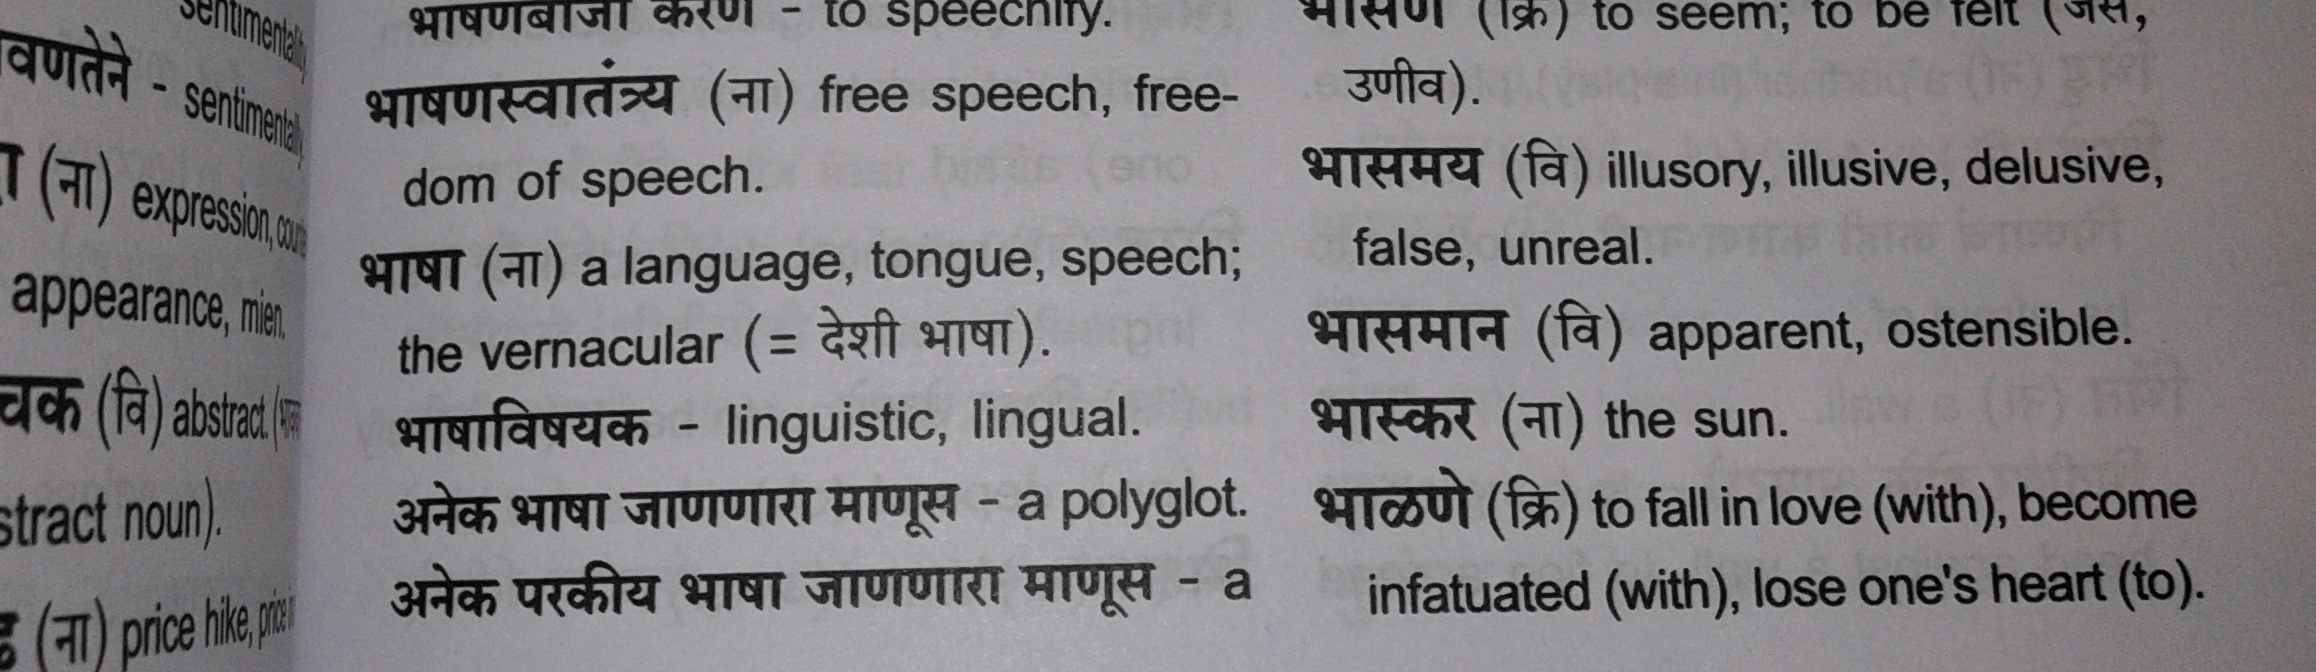
\includegraphics[scale=0.15]{devanagri.jpg}
  \label{script}
\end{figure}
The image in Figure~\ref{script} is an example of Devanagri in a dictionary. \\
\\
Hindi has an SOV grammar and a rich morphology. There are two genders, two numbers, and three cases (direct, oblique, and vocative) for nouns as well as two types of nouns (type-I and type-II) within these categories. Adjectives must agree with nouns in gender, case and number athough some do not decline at all. Verbs are marked with aspect, tense, mood, gender and number \cite{snell}. There are many declensions and conjugations in Hindi, making the development of a morhpological analyzer useful.
\section{Past Work on the Morphology of Hindi}
A seminal work on the grammar and morphology of Hindi is J.T. Platt's ``A grammar of the Hindustani or Urdu language'', written in 1873. In 1997 Rajendra Singh published ``Hindi morphology: a word-based description'', a work that intends to be a mostly comprehensive study of Hindi morphology. Reviewer Alan S. Kaye states that the book is less influential than Platt's and takes issue with a few details of the book. In addition to these, Shaligram Shukla's ``Hindi morphology'' is a good reference for information about Hindi morphology. Smriti Singh has published papers looking at Hindi's nominal and verbal morphology from the Distributed Morphology (DM). Together these resources offer a comprehensive view on the phenomena involved in Hindi morphology.\\
\\
On the system development side of things a few papers have been published concerning building morphological analyzers for Hindi. These papers provide insight on the results and difficulties of building a morphological analyzer for Hindi. They discuss issues surrounding tranlsiteration, visualization, ease of installation and use, morphological modeling (derivational vs. inflectional), and ambiguity (Kanuparthi et. al., 2012; Goyal et. al., 2008; Bögel et al. 2007). Focused on downstream applications like MT, these papers offer a pragmatic view of how to go about modeling Hindi morphology. \\
\section{Available Resources}
Omar N. Koul's ``Modern Hindi Grammar'' is a good Hindi reference grammar that may be useful for understanding the morphological phenomenathat will be supported by this analyzer.
The corpus I have chosen to use is UMC002 English-Hindi. This is a freely available English-Hindi parallel corpus from which I will use the Hindi only. The corpus was created by collecting Hindi from freely available sources such as the ACL 2005 shared task and various web pages. It is a free open source alternative to the EMILLE corpus which is a good resource but not reproducible. The test is in the Devanagari script which is represented in Unicode. Should I decide to transliterate them there are various free lossless transliteration scheme and tools such as ITRANS that are available, though the original script should be fine. I have taken the corpus and created two development corpora of 1000 words each and one test corpus of 10,000 words by filtering out the 12,000 most frequent words and randomly dividing them between A, B, and C. They can be found in the ``corpora'' directory in the repository.
\section{Survey of Phenomena in Hindi}
\subsection{Inflectional:}
\subsubsection{Nouns:}
Hindi nouns are inflected with gender, number, and case. There are three declensions for nouns: masculine nouns ending in आ \emph{/a:/}, all other masculine nouns, and feminine nouns. Inflected nouns are extremely common and as such will be important to cover.
\subsubsection{Pronouns:}
There are personal, demonstrative, relative, possesive, reflexive, interrogative, and indefinite pronouns in Hindi. 
Personal pronouns have two numbers (singular and plural), and three persons, and are inflected for direct, dative, ergative, locative, ablative, and possesive/genitive cases. The second person pronouns can be divided into polite, familiar and intimaite (one of each). The third person pronouns can be divided into proximal and remote (one of each). When personal pronouns are inflected they attach the appropriate postposition as a suffix as well as stem changing (with the exception of the first and second person possessive/genitive forms). It will be important to segment these during morphological analysis.
Other pronouns have only direct and oblique forms, also inflecting for case by stem changing and appending the appropriate postpositions.
\subsubsection{Adjectives:}
There are inflected and uninflected adjectives in Hindi. Inflected adjectives are inflected for gender and number. First and second person possessive pronouns may be used as adjectives that inflect for gender. Numerals may attach two different suffixes to become multiplicatives (e.g. double, threefold, etc.) or aggregates (e.g. both, all three/four/five/etc. of them).
\subsubsection{Verbs:}
Hindi has main and auxiliary verbs.\\
\\
The verb होना \textit{hona} is the copula and has present, past, presumptive, and subjunctive forms.\\
\begin{tabular}{l c l}
होना \textbf{\textit{hona}} & \textbf{:} &\\
Present tense& : &agrees with subject in number and person.\\
Past tense& : &agrees with subject in gender and number.\\
Presumptive form& : &agrees with person, gender and number.\\
Subjunctive form& : &agrees in person and number.\\
\end{tabular}
\\
There are three types of main verbs: simple verbs, conjunct verbs,
and compound verbs. A simple verb may consist of one main verb
and person, gender, number, tense, and aspect markers. In the
compound verb construction, the person, gender, number, and aspect
markers are taken by the explicators/operators, and in the conjunct
verbal construction they are taken by the verb element. The verbal constructions are intransitive, transitive,
ditransitive, causative, dative, conjunct, and compound \cite{koul}.\\
There are four tenses and three aspects. The product of three aspects with four tenses (present, past, presumptive, subjunctive) makes twelve aspectual-tenses. Non-aspectual verb forms include the future, root subjunctive, imperative and infinitive forms. In addition to these tenses and aspects Hindi has three moods: indicative, imperative, and optative. If that's not enough Hindi also has passive, indirect, and ``from/though'' voices, and that just finishes up all the finite verb forms!\\
For non-finite verb forms Hindi has infinitives and perfective, imperfective, and conjunctive participles.\\
All verbal forms will be very important for the analyzer to cover as they are so frequent. Many of these contructions include more than one token as the verbs and explicators are split up. In this iteration of the analyzer I will only handle analysis at the token level. Thus each individual part of a verbal construction is analyzed by itself. Future work can leverage my lexicon and individual analyses to create full verbal analyses.
\subsection{Derivational:}
\subsubsection{Nouns:}
Hindi has a set of of derivational prefixes and suffixes from Persian and Sanskrit that allow for \{noun, adjective, verb\} $\rightarrow$ noun derivations. These may be useful but are lower on the priority list than inflectional morphology.
\subsubsection{Adjectives:}
There are a set of suffixes that allow adjectives to be derived from nouns in Hindi. There are two negative prefixes that also adjective to be derived from adjectives as well. Again, inflectional morphology takes precedence here.
\subsubsection{Adverbs:}
By form, adverbs can be classified into the following subgroups: (a)
basic or non-derived adverbs, (b) derived adverbs, (c) phrasal
adverbs, (d) reduplicated adverbs, and (e) particles.\\
\\
(a) The basic or non-derived adverbs may be either pure adverbs like
आज \textit{a:j} ‘today,’ सदा \textit{sada:}/ हमेशा hameša: ‘always,’ or may be formed
by adding the postposition से \textit{se} to nouns, adjectives, or adverbs.\\
(b) Derived adverbs are formed by adding adverbial suffixes to the
base form of demonstrative, relative, correlative, and interrogative
pronouns. Locative, directional and manner adverbs are formed by adding different suffixes.\\
(c) Phrasal adverbs are formed by adding a simple or a compound
postposition to a noun.\\
(d) Adverbs can be reduplicated to show intensity and distribution.\\
(e) Particles are postpositions that be used to quantify and qualify things like time, weight, frequency, emphasis, etc.
Adverbs would be good to analyze but fall behind nouns, adjectives and verbs in priority.
\section{Initial Design}
The initial design of the system includes the Hindi WordNet database as a lexicon and hand written rules based on the work in \cite{koul}. I present the tagsets for each part of speech below:\\
\subsection{Adjectives}
\subsection{Nouns}
\subsection{Verbs}
\subsection{Pronouns}
\subsection{Postpositions}
\subsection{Adverbs}


\section{System Analysis on Corpus A}

\section{Lessons Learned and Revised Design}

\section{System Analysis on Corpus B}

\section{Final Revisions}

\section{Future Work}


\bibliographystyle{plainnat}
\bibliography{refs}
\label{lastpage}
\end{document}
